\section{Introducing the GUI}
\subsection{Main windows}
Figure~\ref{first look} is a view of the GUI. As you can see there are 4 different windows and three buttons.
\begin{enumerate}
\item The Green window  : This is the window that keeps the text that has already been processed.
\item The Yellow window ': This is the only window you can type your commands into.
\item The Gray  window : this is the Coq feedback window. 
\item The White window : this is a window for messages.
\item The run button: this sends the first line from the input window to Coq.
\item The undo button: this undoes the last command.
\item The draw tree button: this draws the proof trees for all the completed theorems.
\item The symbol buttons: These allows one to type mathematical symbols.
\item The Search box/button: These allow searching for theorems by pattern.
\end{enumerate}


\begin{figure}[h!]
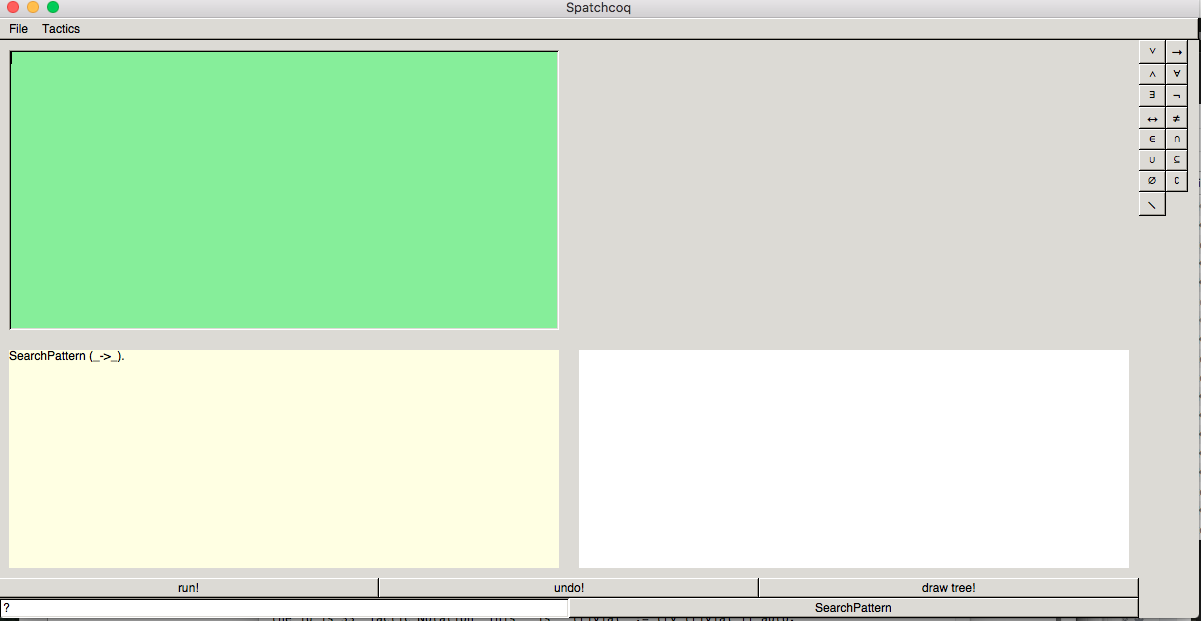
\includegraphics[scale=0.3]{Installation/main.png}
\caption{the GUI}\label{first look}
\end{figure}
\subsection{The menus}

The File menu (Figure \ref{file}) is quite standard:

\begin{figure}[h!]
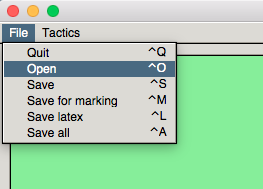
\includegraphics[scale=0.5]{Installation/menu1.png}


\caption{the File  Menu}\label{file}
\end{figure}

The Tactics menu (Figure \ref{tactics}) allows one to pick one of the predefined tactics. 
Note the place keeper VAR. 
These can be modified. More on these later.

\begin{figure}[h!]
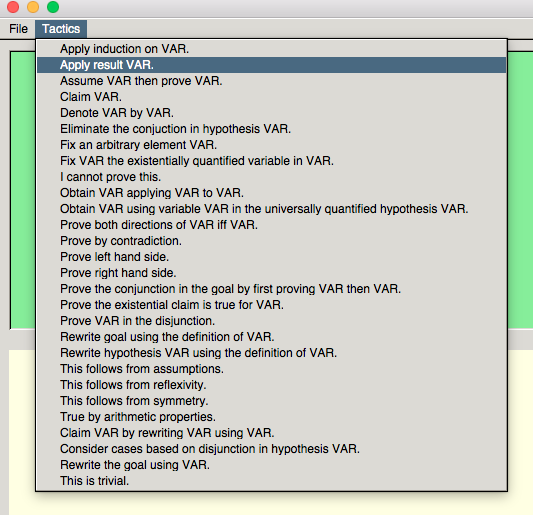
\includegraphics[scale=0.5]{Installation/menu2.png}


\caption{the Tactics/Environment Menus}\label{tactics}
\end{figure}
\subsection{Keyboard shortcuts}

Pressing ESC autocompletes the commands and pressing \VAR circles around the various possibilities for VAR.



